%\documentclass[12pt]{report}
%\documentclass[12pt]{extreport}
\documentclass[17pt]{extarticle}
\usepackage{graphicx}
\usepackage{setspace}
\usepackage{amsmath,amssymb}
\usepackage{IEEEtrantools}
\usepackage{cancel}
\usepackage[font=small,labelfont=bf]{caption}

\usepackage{geometry}
 \geometry{
 a4paper,
 total={170mm,264mm},
 left=20mm,
 top=10mm,
 }

\begin{document}

\section{Notazioni vettoriali}

Se poniamo un sistema di riferimento cartesiano (x, y, z), come in figura \ref{fig:ternaCartesiana}	) e se consideriamo soltanto quei vettori con punto di applicazione coincidente con l'origine, allora ad ogni punto dello spazio associo un vettore e viceversa. Di conseguenza, in queste circostanze, possiamo identificare anche un vettore (e non soltanto un punto) con una sequenza ordinata di 3 numeri. In questo contesto le parole "punto" e "vettore" vengono usate pressoch\'e come sinonimi.



\begin{figure}[b!]		
	\centering
   	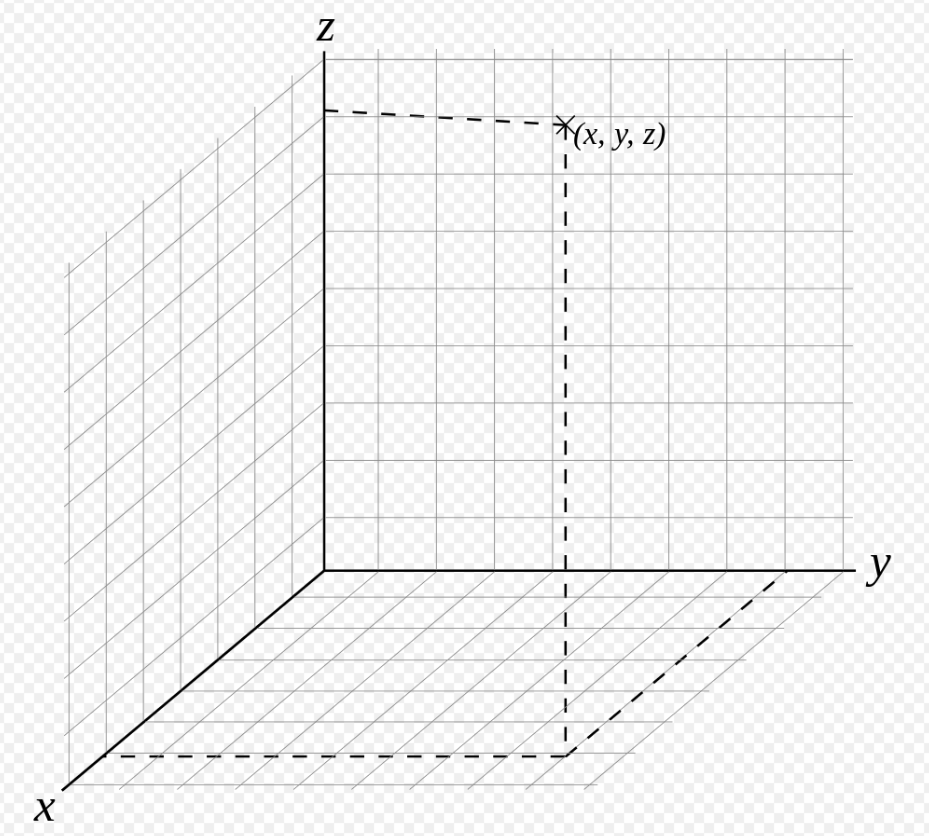
\includegraphics[width=3.4in]{SistemaRifCartesiano.png}		%rettaNONpassOrig.jpg
  	\caption{Sistema di riferimento cartesiano}
   	\label{fig:ternaCartesiana}
\end{figure}


Il {\bf versore} \'e un vettore di modulo unitario che viene utilizzato per identificare una specifica direzione nello spazio. Tipicamente un versore viene scritto con un "cappuccietto" sopra la lettera. In particolare, dato un sistema di riferimento x, y e z, si usano i seguenti simboli
\begin{itemize}
	\item $\hat{i}$ versore parallelo e concorde all'asse x
	\item $\hat{j}$ versore parallelo e concorde all'asse y
	\item $\hat{k}$ versore parallelo e concorde all'asse z
\end{itemize}

Quindi, un vettore o un punto possono essere scritti, oltre che con la classica espressione $\vec{v} = (x, y, z)$ anche con la seguente dicitura:

\begin{eqnarray}
	\vec{v} & = & x\hat{i} + y\hat{j} + z\hat{k}
\end{eqnarray}


Ad esempio, un punto nel piano distante 3 dall'asse x e -4 dall'asse y sar\'a scritto nel seguente modo:

\begin{eqnarray}
	\vec{v} & = & -4\hat{i} + 3\hat{j}
\end{eqnarray}
un punto nello spazio distante 3 dal piano yz, 4 dal piano xz e -5 dal piano xy, pu\'o essere scritto nel seguente modo:

\begin{eqnarray}
	\vec{v} & = & 3\hat{i} + 4\hat{j} - 5\hat{k}
\end{eqnarray}


\section{Prodotto scalare}

Il prodotto scalare tra due generici vettori $\vec{a}$ e $\vec{b}$, come in figura \ref{fig:prodScalare}, \'e definito come quel numero $p$ pari al prodotto del modulo $a$ del vettore $\vec{a}$, per il modulo $b$ del vettore $\vec{b}$ per il coseno dell'angolo compreso.
\begin{eqnarray}\label{eq:prodScal}
	p = \vec{a}\cdot\vec{b} = ab\cos\gamma
\end{eqnarray}

\begin{figure}[h]	
	\centering
   	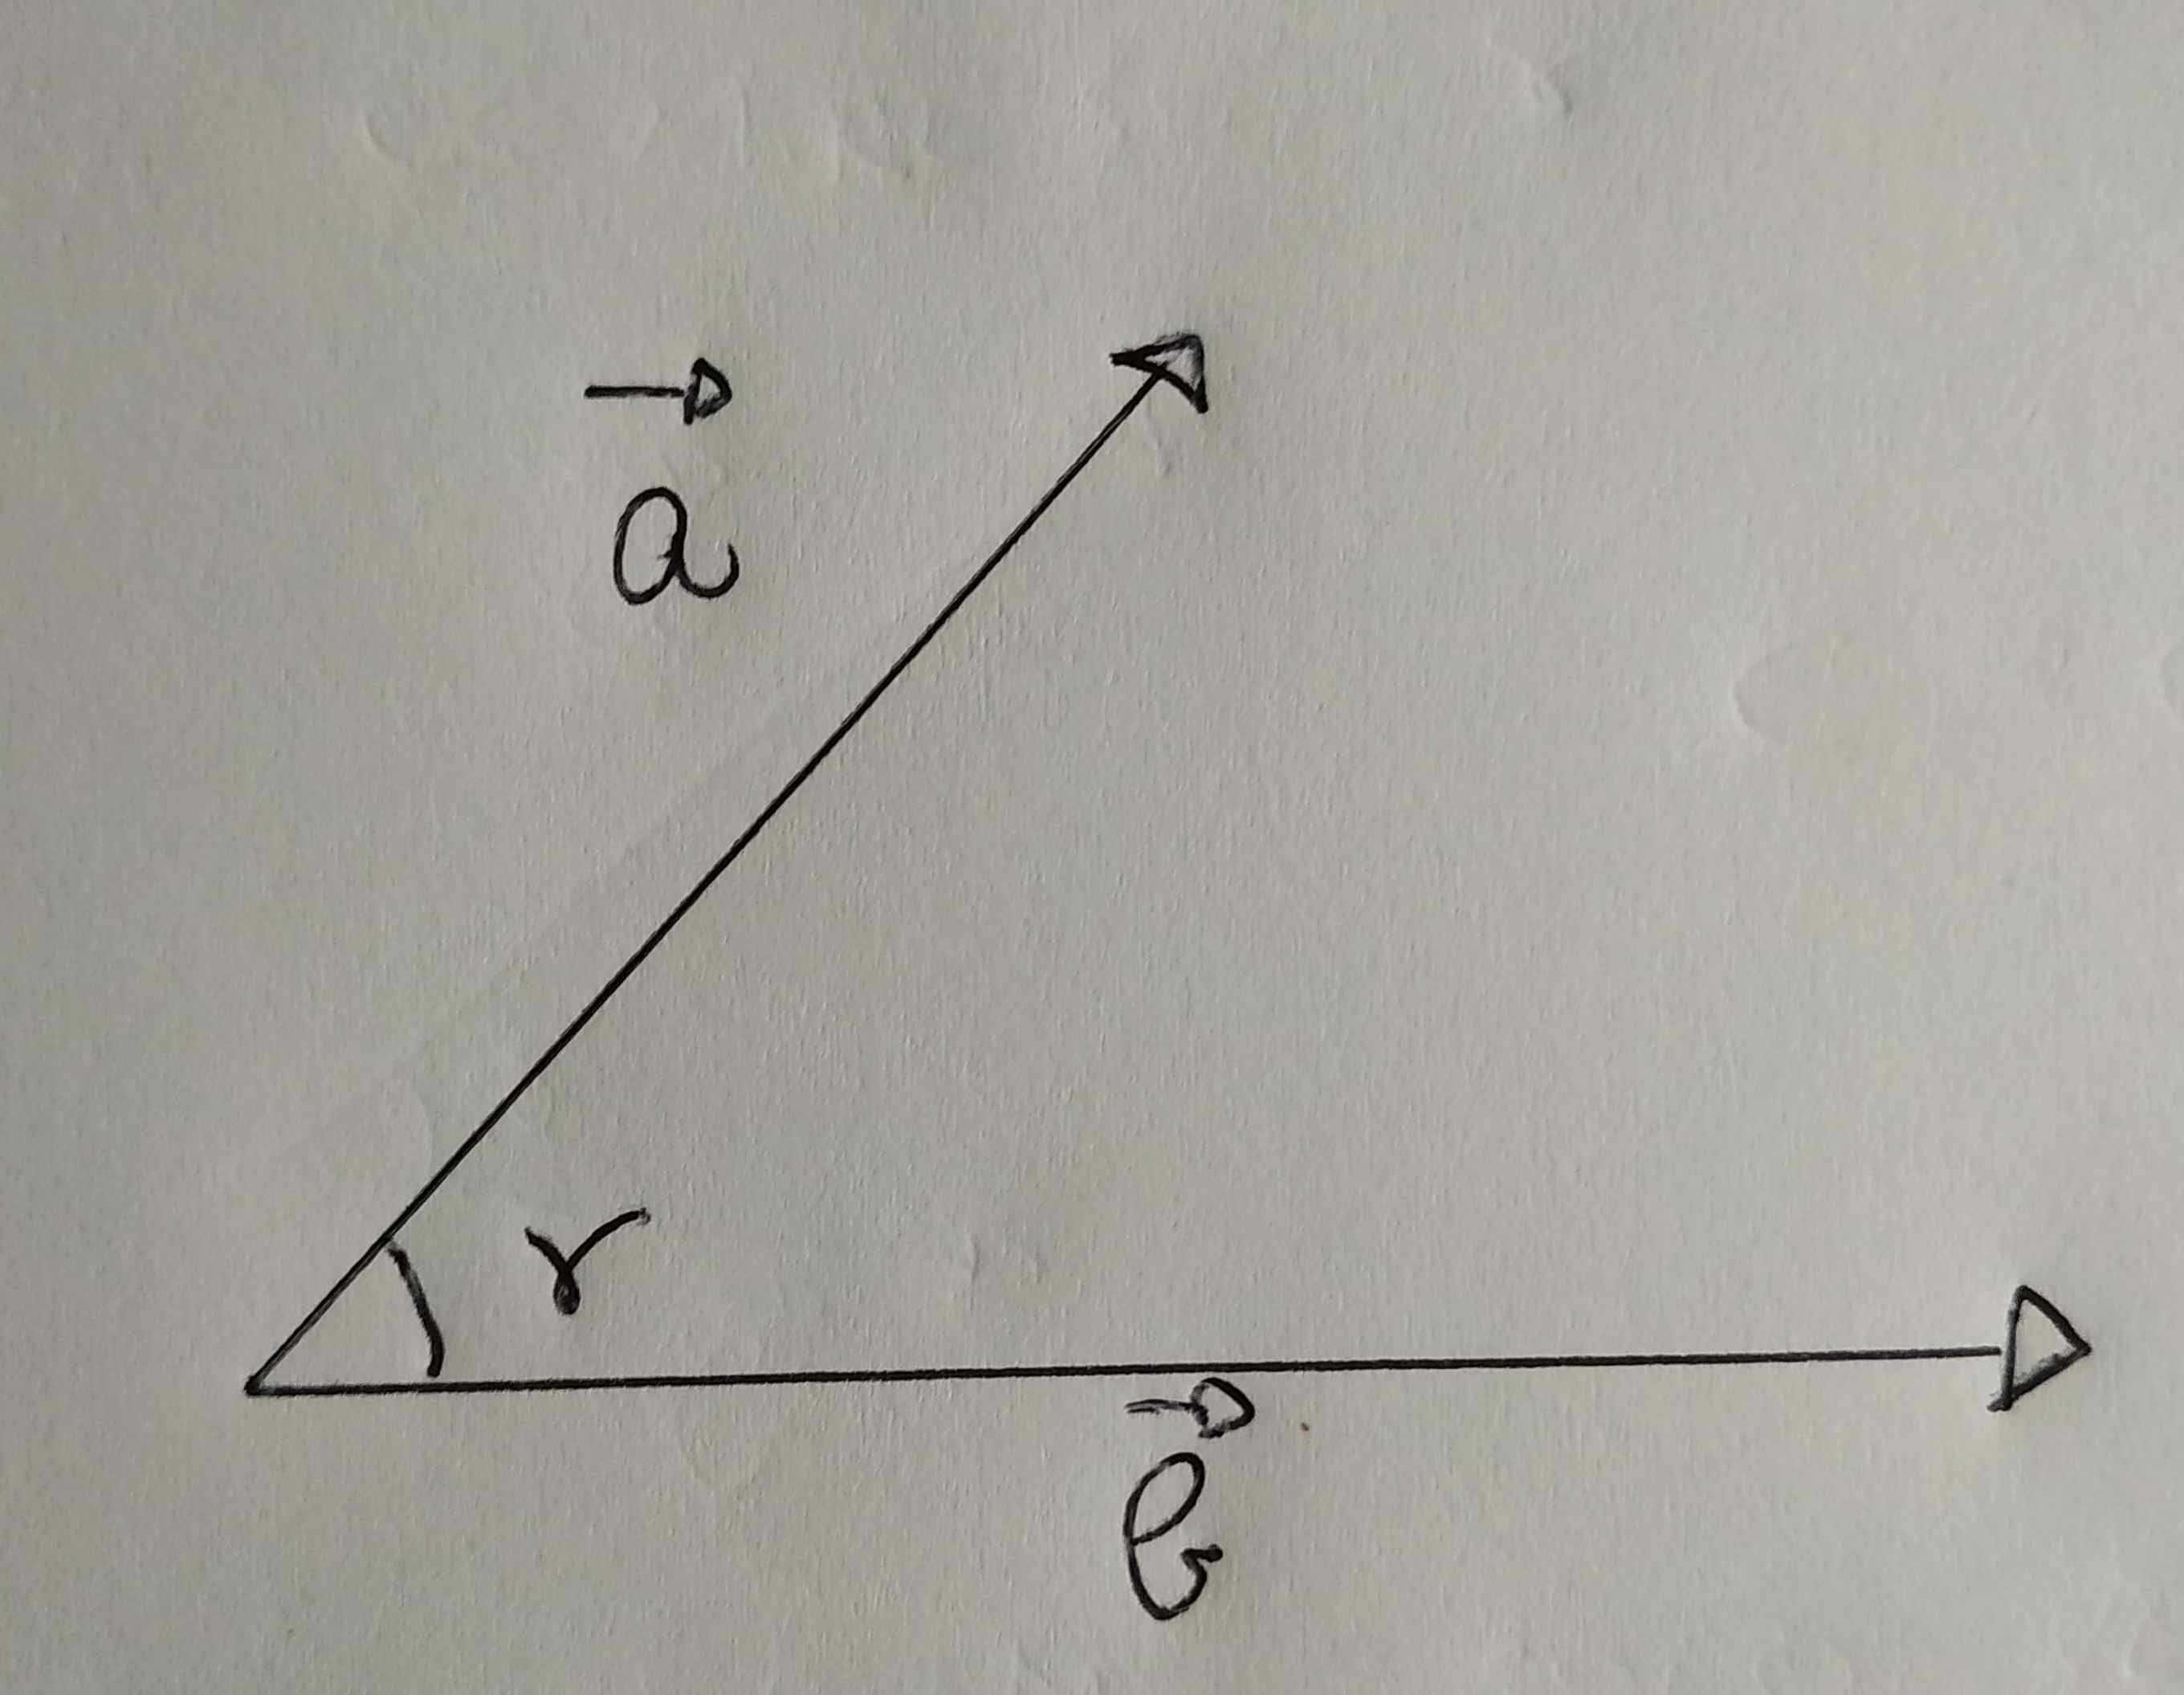
\includegraphics[width=2.5in]{ProdottoScalare.jpg}%eqRetta.jpg
   	\caption{Prodotto scalare}
   	\label{fig:prodScalare}		
\end{figure}

Dato un sistema di riferimento cartesiano come in figura \ref{fig:ternaCartesiana}, e due vettori $\vec{a}$ e $\vec{b}$  

\begin{eqnarray}
	\vec{a} & = & a_x\hat{i} + a_y\hat{j} + a_z\hat{k}\\
	\vec{b} & = & b_x\hat{i} + b_y\hat{j} + b_z\hat{k}
\end{eqnarray}

si dimostra che il loro prodotto scalare \'e la somma dei prodotti delle rispettive coordinate:
\begin{eqnarray}\label{eq:prodScalCart}
	p = a_xb_x + a_yb_y + a_zb_z
\end{eqnarray}

Se i due vettori sono disposti in un piano, anzich\'e nello spazio, allora l'equazione \ref{eq:prodScalCart} risulta semplificata come segue:

\begin{eqnarray}\label{eq:prodScalCart2}
	p = a_xb_x + a_yb_y
\end{eqnarray}


\section{Equazione della retta e del piano con il prodotto scalare.}

Dalla equazione \ref{eq:prodScal}, si evince che il prodotto scalare di due vettori $\vec{a}$ e $\vec{b}$ paralleli tra loro \'e massimo e pari a $p = ab$, mentre il prodotto scalare di due vettori tra loro ortogonali \'e nullo. 

Quindi, dato un piano, un sistema di riferimento (x, y) e un vettore $\vec{v} = v_x\hat{i} + v_y\hat{j}$ (fig \ref{fig:eqRetta}), possiamo usare l'operazione di prodotto scalare (equazione \ref{eq:prodScalCart2}) per identificare il luogo geometrico di tutti e soli i punti di coordinate x ed y, perpendicolari al vettore $\vec{v}$:

\begin{eqnarray}
	p = v_xx + v_yy = 0
\end{eqnarray}
tale luogo geometrico \'e una retta \emph{passante} per l'origine e con coefficiente angolare $m = -v_x/v_y$. 

\begin{figure}[h]	
	\centering
   	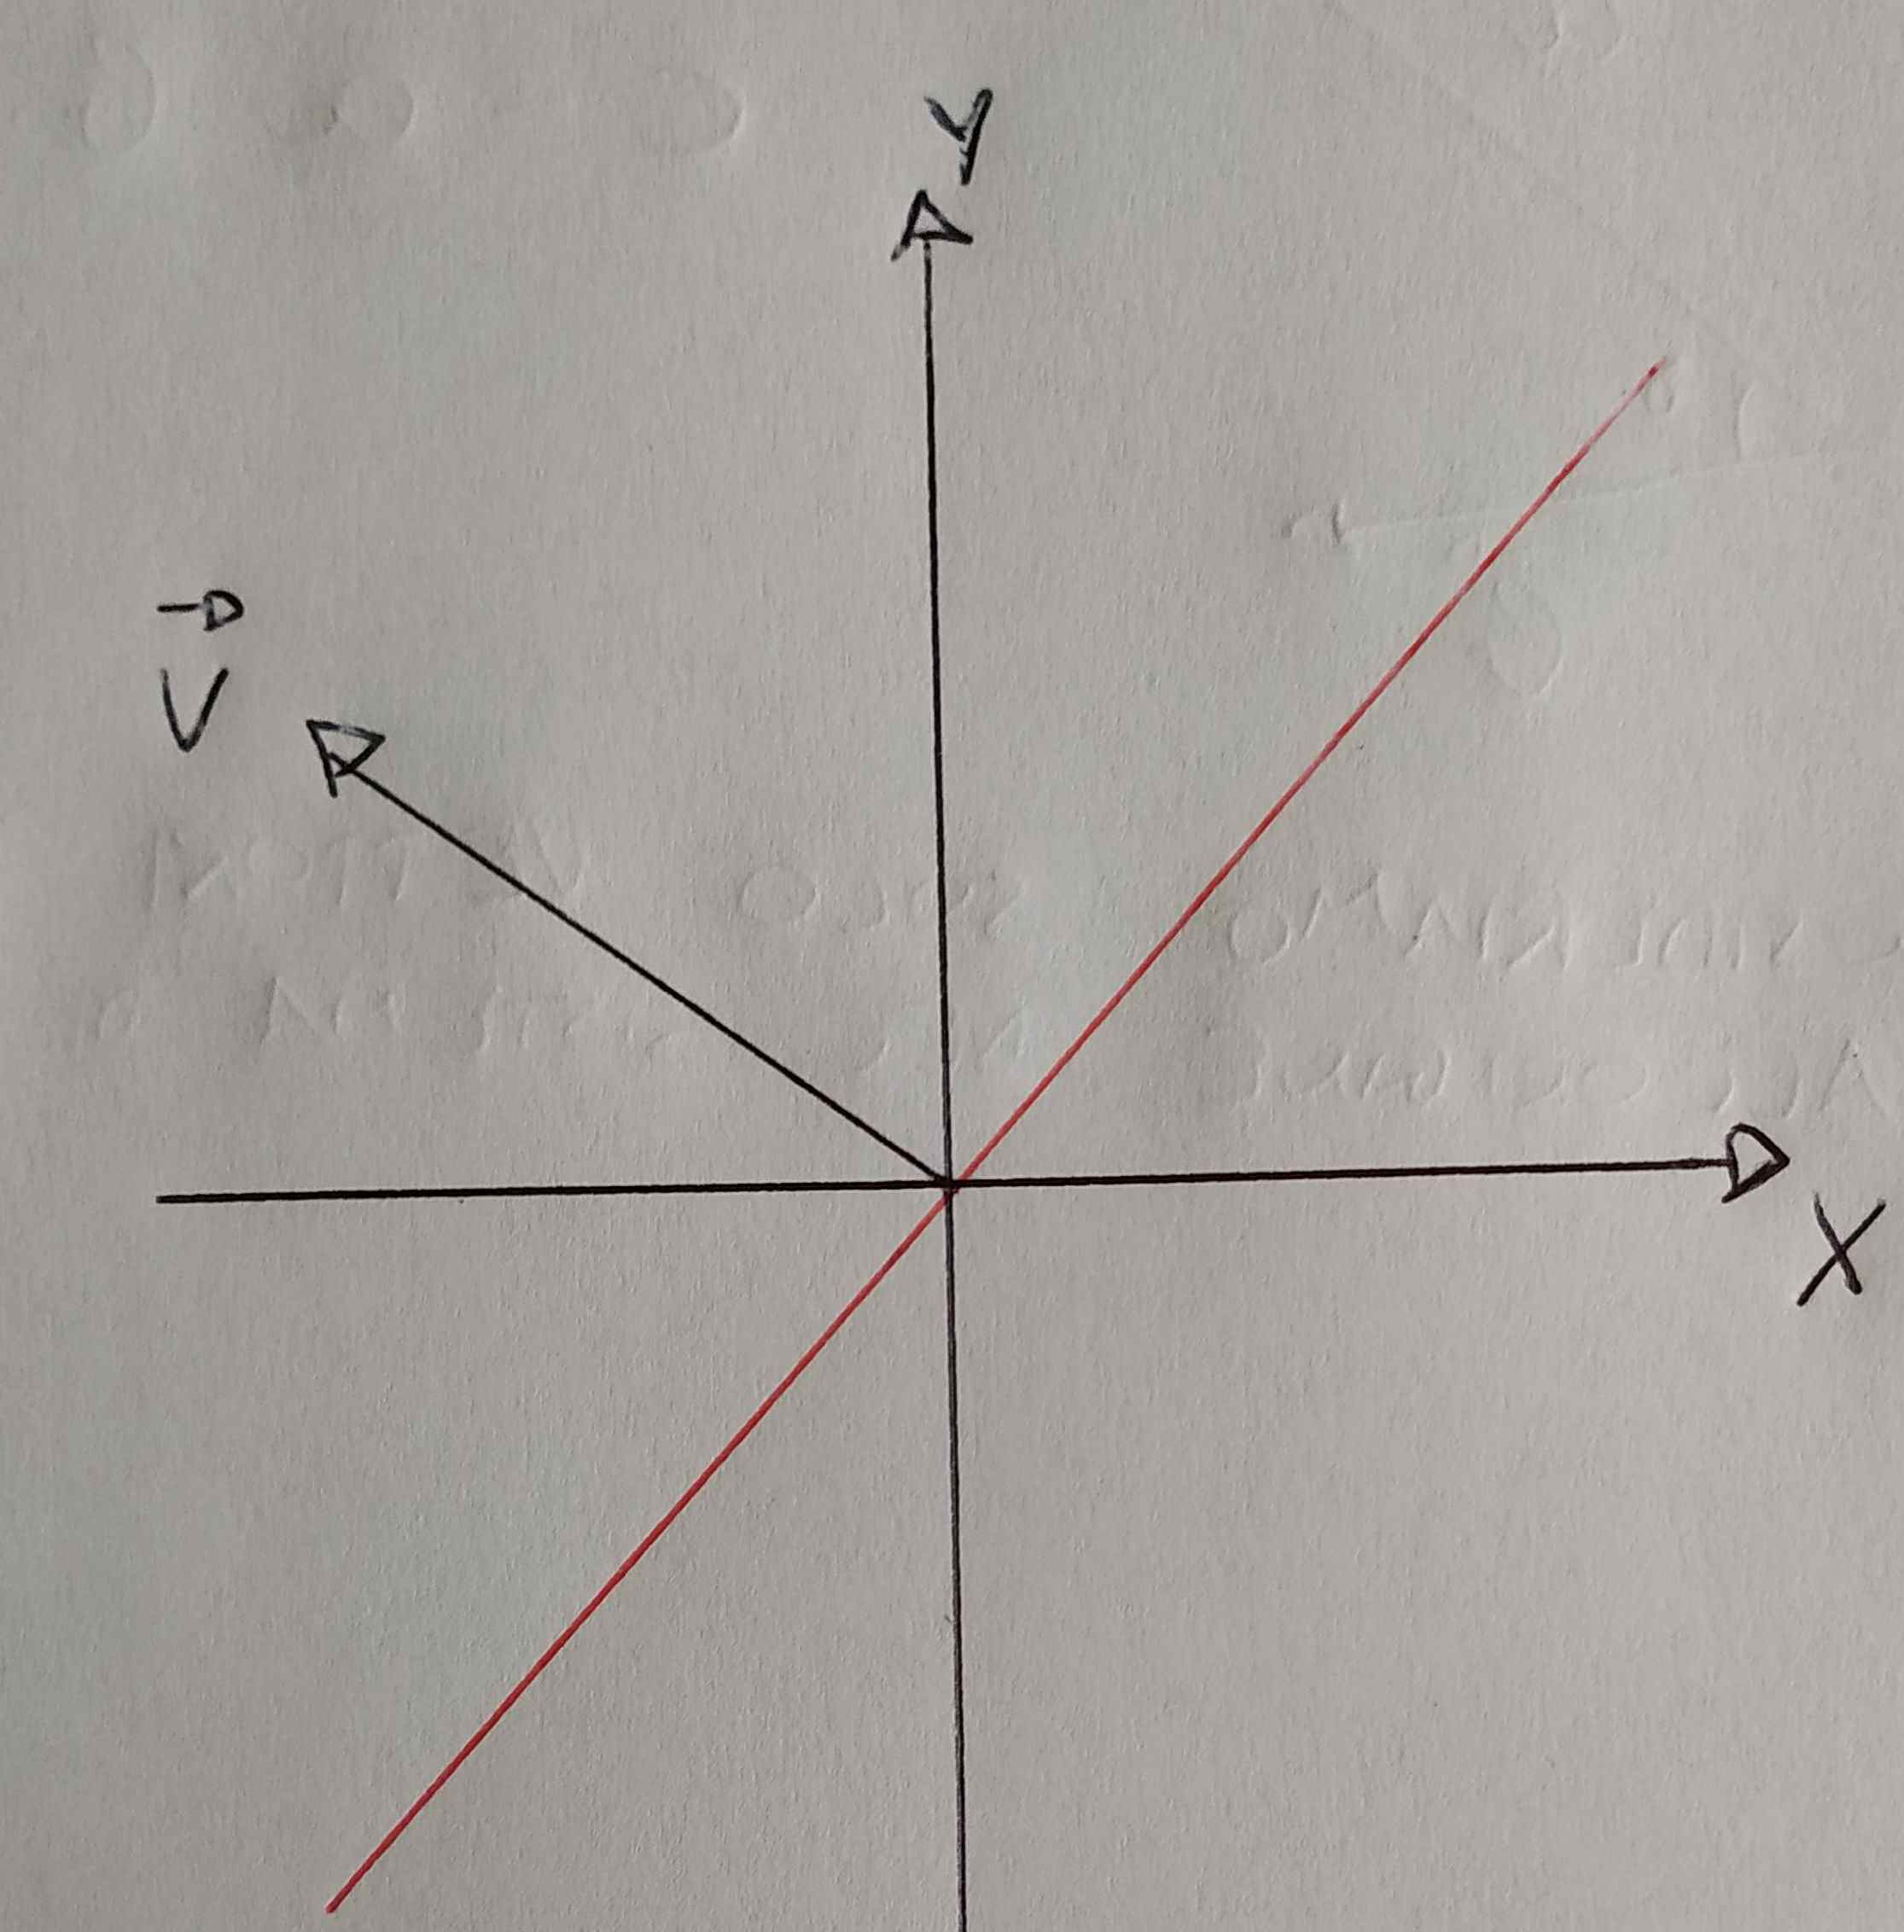
\includegraphics[width=2.5in]{eqRetta.jpg}
   	\caption{Retta (linea rossa) perpendicolare a un vettore $\vec{v}$}
   	\label{fig:eqRetta}		
\end{figure}

Anche l'equazione di una retta \emph{non passante} per l'origine pu\'o esser ricavata con il prodotto scalare. Infatti, ciascun punto P(x, y) di una tale retta pu\'o esser ''raggiunto'' sommando vettorialmente due vettori, come in figura \ref{fig:rettaNONpassOrig}. Il vettore $\vec{p} - \vec{a}$, di cui $\vec{a} = a\hat{j}$ \'e noto ed identifica l'intercetta e $\vec{p} = x\hat{i} + y\hat{j}$ \'e incognito, prodotto scalarmente con un vettore $\hat{v}$ ortogonale ad esso, da luogo all'equazione di una retta con intercetta differente da zero



\begin{figure}[b!]		
	\centering
   	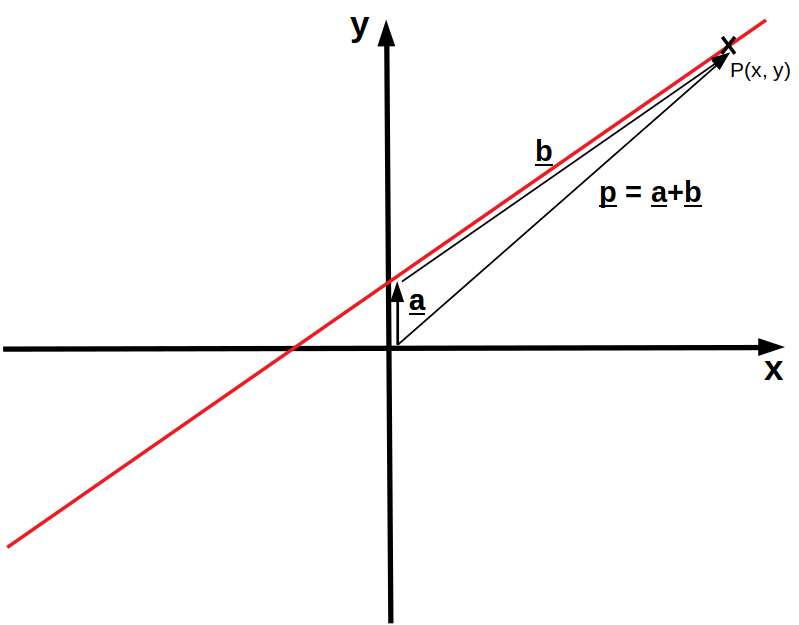
\includegraphics[width=3.0in]{rettaNONpassOrig.jpg}		%
  	\caption{Ciascun punto P(x, y), appartenente a una retta NON passante per l'origine, pu\'o essere "raggiunto" tramite la somma di due vettori: uno congiungente l'origine con l'intercetta e l'altro congiungente l'intercetta con il punto stesso.}
   	\label{fig:rettaNONpassOrig}
\end{figure}


\begin{eqnarray}\label{eq:prodScalX}
	(\vec{p} -\vec{a})\cdot \hat{v} = 0
\end{eqnarray}

Infatti, usando per l'equazione \ref{eq:prodScalX} la sua espressione in termini delle componenti cartesiane, si ha

\begin{eqnarray}
	(x\hat{i} + y\hat{j} -a\hat{j})\cdot (v_x\hat{i} + v_y\hat{j} ) = 0
\end{eqnarray}

e, una volta sviluppata si ottiene

\begin{eqnarray}\label{eq:Rettau}
	xv_x+yv_y + av_x = 0
\end{eqnarray}







%\section{Equazione di una piano e prodotto scalare.}

Dato uno spazio, un sistema di riferimento (x, y, z) e un vettore $\vec{v} = v_x\hat{i} + v_y\hat{j} + v_z\hat{k}$, possiamo usare l'operazione di prodotto scalare (equazione \ref{eq:prodScalCart}) per identificare il luogo geometrico di tutti e soli i vettori di coordinate x, y e z, perpendicolari al vettore $\vec{v}$:






\begin{eqnarray}
	p = v_xx + v_yy + v_zz = 0
\end{eqnarray}


Tale luogo geometrico \'e rappresentato da un piano.

Da ci\'o si osserva anche la seguente cosa: mentre l'equazione
\begin{eqnarray}
	ax + by + c = 0
\end{eqnarray}
rappresenta una retta nel piano. L'equazione 

\begin{eqnarray}
	ax + by + cz + d = 0
\end{eqnarray}
rappresenta un piano nello spazio.





Inoltre, esattamente come un punto nel piano pu\'o esser espresso per mezzo del sistema delle equazioni di due rette
\begin{IEEEeqnarray}{lCr}
 {\setstretch{2.25}%Distance between two following lines
\left\{ \begin{array}{ccc}
a_1x + b_1x + c_1 & = & 0 \\ 
a_2x + b_2x + c_2 & = & 0
\end{array}
\right. } \label{eq:sistema}
\end{IEEEeqnarray} 

 cos\'i una retta nello spazio pu\'o essere espressa per mezzo di un sistema di due equazioni del piano nello spazio



\begin{IEEEeqnarray}{lCr}
 {\setstretch{2.25}%Distance between two following lines
\left\{ \begin{array}{ccc}
a_1x + b_1x + c_1z + d_1 & = & 0 \\ 
a_2x + b_2x + c_2z + d_1 & = & 0
\end{array}
\right. } \label{eq:sistema}
\end{IEEEeqnarray} 




\section{Onde}





L'equazione di un onda piana che si propaga in direzione $x$, cos\'i come trattata nel capitolo 1 \'e

\begin{eqnarray}
	y = A\sin\left(kx - \omega t + \phi\right)
\end{eqnarray}

Il termine $kx$ della fase \'e un prodotto scalare tra due vettori paralleli: il vettore d'onda $\vec{k}$ e il vettore posizione $\vec{x}$. Pi\'u in generale, il vettore posizione pu\'o trovarsi in qualsiasi punto dello spazio, identificato da un generico vettore $\vec{r} = x\hat{i} + y\hat{j} + z\hat{k}$ e i due vettori $\hat{k}$ e $\hat{r}$ possono NON essere paralleli. L'equazione dell'onda si dovr\'a quindi scrivere:  


\begin{eqnarray}
	y = A\sin\left(\vec{k}\cdot\vec{r} - \omega t + \phi\right)
\end{eqnarray}



\end{document}